\documentclass[12pt]{article}
\usepackage{amsmath}
\usepackage{amssymb}
\usepackage[letterpaper,margin=0.85in,centering]{geometry}
\usepackage{fancyhdr}
\usepackage{enumerate}
\usepackage{lastpage}
\usepackage{multicol}
\usepackage{graphicx}
\usepackage{hyperref}

\reversemarginpar

\pagestyle{fancy}
\cfoot{}
\lhead{Math 1410}\chead{Worksheet \# 1 Solutions}\rhead{Tuesday, 12\textsuperscript{th} January, 2016}
%\rfoot{Total: 10 points}
%\chead{{\bf Name:}}
\newcommand{\points}[1]{\marginpar{\hspace{24pt}[#1]}}
\newcommand{\skipline}{\vspace{12pt}}
%\renewcommand{\headrulewidth}{0in}
\headheight 30pt

\newcommand{\di}{\displaystyle}
\newcommand{\abs}[1]{\lvert #1\rvert}
\newcommand{\len}[1]{\lVert #1\rVert}
\renewcommand{\i}{\mathbf{i}}
\renewcommand{\j}{\mathbf{j}}
\renewcommand{\k}{\mathbf{k}}
\newcommand{\R}{\mathbb{R}}
\newcommand{\aaa}{\mathbf{a}}
\newcommand{\bbb}{\mathbf{b}}
\newcommand{\ccc}{\mathbf{c}}
\newcommand{\dotp}{\boldsymbol{\cdot}}
\newcommand{\bbm}{\begin{bmatrix}}
\newcommand{\ebm}{\end{bmatrix}}                   
                  
\begin{document}


%\author{Instructor: Sean Fitzpatrick}
\thispagestyle{fancy}
%\noindent{{\bf Name and student number:}}
 \begin{enumerate}
 \item  Let $P=(1,0,-2)$, $Q=(-3,2,4)$, and $R=(0,5,-1)$ be points in $\R^3$.
\begin{enumerate}
 \item Calculate the vectors $\vec{u}=\overrightarrow{PQ}$, $\vec{v}=\overrightarrow{QR}$, and $\vec{w}=\overrightarrow{PR}$.

\bigskip

To find the components of a vector between two points, we subtract the coordinates of the initial point from the coordinates of the final point. Therefore,
\[
 \vec{u} = \bbm -3-1\\2-0\\4-(-2)\ebm = \bbm -4\\2\\6\ebm \quad \vec{v} = \bbm 0-(-3)\\5-2\\-1-4\ebm = \bbm 3\\3\\-5\ebm \quad \vec{w} = \bbm 0-1\\5-0\\-1-(-2)\ebm = \bbm -1\\5\\1\ebm.
\]


 \item Show that $\vec{u}+\vec{v} = \vec{w}$.

\bigskip

To add vectors we add the corresponding components; therefore,
\[
 \vec{u}+\vec{v} = \bbm -4\\2\\6\ebm+\bbm 3\\3\\-5\ebm = \bbm -4+3\\2+3\\6-5\ebm = \bbm -1\\5\\1\ebm = \vec{w}.
\]


 \item Explain, with a diagram, why your result in part (b) makes sense. (You do not have to accurately plot the points $P,Q,R$.)

\begin{multicols}{2}
 An inaccurate plot is given on the right. (The points $P,Q,R$ don't reflect their true coordinates, but given these points, the vectors are drawn correctly.) It makes sense that $\vec{u}+\vec{v}=\vec{w}$, since $\vec{w}$ represents travelling directly from $P$ to $R$, while the tip-to-tail rule for adding $\vec{u}$ and $\vec{v}$ can be thought of as travelling from $P$ to $R$ with a detour via the point $Q$.

For an accurate (and interactive) plot of the three points and the corresponding vectors, see 
\href{http://tube.geogebra.org/m/g1ivjhY4}{http://tube.geogebra.org/m/g1ivjhY4}.

\columnbreak
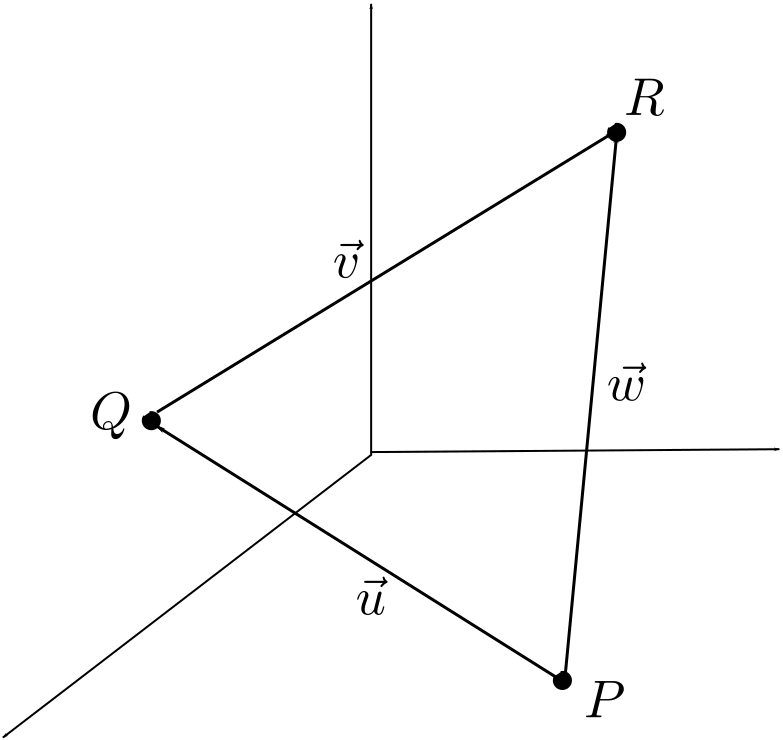
\includegraphics[width=\columnwidth]{WS1-1(c)}
\end{multicols}

\end{enumerate}


\item Let $\vec{a} = \begin{bmatrix}1\\4\\-7\end{bmatrix}$ and $\vec{b} = \begin{bmatrix}-3\\5\\2\end{bmatrix}$.

\medskip

Find the vector $\vec{c}$ given by the linear combination $\vec{c} = 4\vec{a}-3\vec{b}$.

\bigskip

Using the definitions of addition and scalar multiplication of vectors, we have
\[
 \vec{c} = 4\vec{a}-3\vec{b} = 4\bbm 1\\4\\-7\ebm - 3\bbm -3\\5\\2\ebm = \bbm 4\\16\\-28\ebm +\bbm 9\\-15\\-6\ebm = \bbm 4+9\\16-15\\-28-6\ebm = \bbm 13\\1\\-34\ebm.
\]
Note: the calculation above {\em added} the vectors $4\vec{a}$ and $-3\vec{b}$ but you could equally well subtract the vectors $4\vec{a}$ and $3\vec{b}$.

\bigskip

\item Let $\vec{u} = \bbm 1\\2\ebm$ and let $\vec{v} = \bbm -2\\1\ebm$ be vectors in $\R^2$. Sketch the vectors $\vec{u}, \vec{v}$, and $3\vec{u}-2\vec{v}$.

\bigskip

We plot all three vectors in their standard positions (with tails at the origin). Note that
\[
 3\vec{u}-2\vec{v} = 3\bbm 1\\2\ebm-2\bbm -2\\1\ebm = \bbm 3\\6\ebm + \bbm 4\\-2\ebm = \bbm 7\\4\ebm.
\]
\begin{center}
 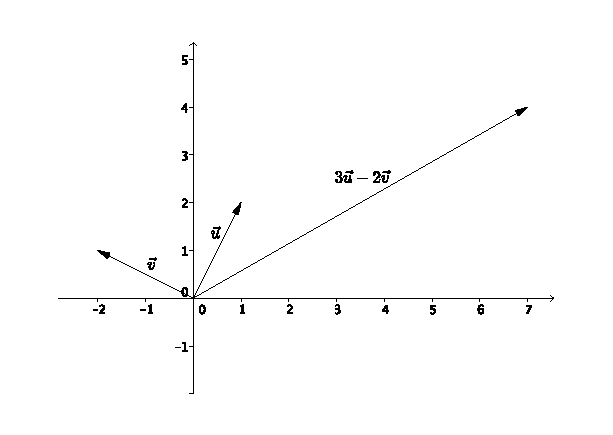
\includegraphics[width=5in]{WS1-3}
\end{center}

\item Recall that the {\em absolute value} function $\abs{x}$ is defined by
\[
 \abs{x} = \begin{cases} x, & \text{ if } x\geq 0\\ -x, & \text{ if } x<0\end{cases}.
\]
\begin{enumerate}
 \item Calculate $\abs{2}$, $\abs{3.5}$, $\abs{0}$, $\abs{-5}$, and $\abs{-7/4}$.

\bigskip

Since $2\geq 0$, the definition of $\abs{x}$ gives $\abs{2}=2$. Simlarly, $3.5\geq 0$ and $0\geq 0$, so $\abs{3.5}=3.5$ and $\abs{0}=0$.

Since $-5<0$, the definition of $\abs{x}$ gives $\abs{-5} = -(-5) = 5$, and similarly, $\abs{-7/4} = -(-7/4) = 7/4$.

\bigskip

 \item Explain in your own words what the effect of $\abs{x}$ is on a real number $x$.

\bigskip

If $x=0$ or $x$ is a positive real number, then $\abs{x}=x$, so the absolute value function does nothing.

If $x$ is a negative real number, then $\abs{x} = -x$, so the absolute value function switches the sign to give the corresponding positive number.

\bigskip

 \item Calculate $\sqrt{(2^2)}$, $\sqrt{(0)^2}$, $\sqrt{(-1)^2}$ and $\sqrt{(-2)^2}$. 

\bigskip

We have $\sqrt{2^2} = \sqrt{4} = 2$, $\sqrt{0^2} = \sqrt{0} = 0$, $\sqrt{(-1)^2} = \sqrt{1} = 1$, and $\sqrt{(-2)^2} = \sqrt{4} = 2$.

\bigskip

 \item Explain why it's true that $\sqrt{x^2} = \abs{x}$ for any real number $x$.

\bigskip

Generalizing from the examples above, we can see that whenever $x\geq 0$, $\sqrt{x^2} = x$, whereas if $x$ is negative, the square root function (which is never negative) gives us back not $x$, but the corresponding positive number, which is $-x$. This is exactly the same as our description of the absolute value function in part (b) above.

\bigskip

 \item Let $\vec{v} = \begin{bmatrix}x\\y\\z\end{bmatrix}$ be a vector in $\R^3$, and let $c\in \R$ be any scalar. Recall that $\len{\vec{v}}$ is defined by
\[
 \len{\vec{v}} = \sqrt{x^2+y^2+z^2}.
\]
Show that $\len{c\vec{v}} = \abs{c}\len{\vec{v}}$. How is this related to the geometric interpretation of scalar multiplication?

\bigskip

By the algebraic definition of scalar multiplication, we have $c\vec{v} = c\bbm x\\y\\z\ebm = \bbm cx\\cy\\cz\ebm$, so using the definition of the magnitude of a vector given above,
\begin{align*}
 \len{c\vec{v}} & = \sqrt{(cx)^2+(cy)^2+(cz)^2}\\
& = \sqrt{c^2x^2+c^2y^2+c^2z^2}\\
& = \sqrt{c^2(x^2+y^2+z^2)}\\
& = \sqrt{c^2}\sqrt{x^2+y^2+z^2}\\
& = \abs{c}\len{\vec{v}},
\end{align*}
which is what we needed to show. (In the last step, we used the definition of $\len{\vec{v}}$ given above, and the result from part (d).)

\medskip

One final note of caution: a common algebraic error is to treat the square root function as if it were a linear function. Since $(x+y)^2 = x^2+2xy+y^2 \neq x^2+y^2$, it's also true that $\sqrt{x+y}\neq \sqrt{x}+\sqrt{y}$. (If these were in fact equal, the Pythagorean Theorem would not be very interesting.) For example, $\sqrt{3^2+4^2} = \sqrt{9+16} = \sqrt{25}=5$. This is {\bf not} equal to $\sqrt{3^2}+\sqrt{4^2} = 3+4=7.$
\end{enumerate}

 \end{enumerate}
\end{document}